%----------------------------------------------------------------------------------------------------------------------

\documentclass[a4paper,12pt]{report}
\usepackage[utf8]{inputenc}
\usepackage[portuguese]{babel}
\usepackage{graphicx}
\usepackage{hyperref}
\usepackage{float}
\usepackage{listings}
\usepackage{longtable}
\usepackage{subfig}
\usepackage{tabularx}
\usepackage[table,xcdraw]{xcolor}
\usepackage{adjustbox}
\newcommand*{\xml}[1]{\texttt{<#1>}}
\usepackage[T1]{fontenc}
\usepackage{lmodern}
\newcommand*{\escape}[1]{\texttt{\textbackslash#1}}
\newcommand*{\escapeI}[1]{\texttt{\expandafter\string\csname #1\endcsname}}
\newcommand*{\escapeII}[1]{\texttt{\char`\\#1}}
\usepackage[bottom]{footmisc}


%----------------------------------------------------------------------------------------------------------------------

\usepackage{geometry}
 \geometry{
     a4paper,
     total={170mm,257mm},
     left=30mm,
     right=25mm,
     top=30mm,
     bottom=25mm,
 }

\graphicspath{{./base_images/}}

%----------------------------------------------------------------------------------------------------------------------

\begin{document}

%----------------------------------------------------------------------------------------------------------------------


\begin{titlepage}
    \center
    {

    \begin{figure}[t]
        \centering
        
\includegraphics[scale=0.4]{images/uminho.png}
        \label{img:logo}
        \vspace{2.0cm}
    \end{figure}

    \vspace{3.0cm}
    \textsc{\Huge \textbf{Programação em Lógica Estendida, Métodos de Resolução de Problemas e de Procura}}\\[1.5cm]
    \textsc{\Large Sistemas de Representação de Conhecimento e Raciocínio}\\[1.5cm]
    \textsc{Mestrado Integrado em Engenharia Informática}\\[0.2cm]
    \textsc{(2019/2020)}
    
    \vspace{5cm}
    \begin{flushleft}

        \vspace{1cm}
        \large 
        \vspace{0.5cm}
        A83719 \,\,\,Pedro Machado
        \vspace{0.2cm}
    \end{flushleft}
    \begin{flushright}
        Braga

        Junho 2020
    \end{flushright}

\date{\today}
}
\end{titlepage}


\begin{abstract}
    O trabalho desenvolvido pretendia abordar a programação em lógica através do \textbf{PROLOG} e de métodos de resolução de problemas e de procura. Assim, era pretendido desenvolver um sistema capaz de armazenar conhecimento relativo aos transportes públicos do concelho de Oeiras e possibilitar a recomendação de trajetos a percorrer.
    \par Ao longo deste relatório vai-se proceder à descrição do trabalho realizado bem como a  sua metodologia. Assim, proceder-se-á a uma breve explicação dos algoritmos desenvolvidos, predicados usados e, de seguida, uma explicação da metodologia aplicada no desenvolvimento das funcionalidades do sistema. Por último, será demonstrado uma breve comparação de resultados e análise destes.
    \par Em suma, acho que o trabalho desenvolvido cumpre os objetivos propostos pela equipa docente e que este possibilitou a uma melhor assimilação de conhecimentos teóricos e práticos dados pela cadeira de Sistemas de Representação de Conhecimento e Raciocínio, bem como da programação lógica em \textbf{PROLOG}. 
\end{abstract}



\renewcommand*\contentsname{Índice}
\renewcommand{\bibname}{Referências}

%Indice
\tableofcontents
\clearpage


% Introdução

\chapter{Introdução}

Este relatório é relativo ao trabalho prático individual da UC de Sistemas de Representação de Conhecimento e Raciocínio que tem como objetivos a motivação para o uso de linguagens lógicas, usando a linguagem de programação em lógica \textbf{PROLOG}, no âmbito de métodos de Resolução de Problemas e no desenvolvimento de algoritmos de pesquisa.
\vspace{0.3cm}
\par O caso de estudo deste trabalho incide na utilização de transportes públicos no concelho de Oeiras. Assim, era necessário ter em conta as informações relativas às paragens de autocarro de Oeiras, bem como as suas características, tais como a sua localização, as carreiras que as utilizam e respetivas operadoras, entre outras.
\par Desta forma, era pretendido o desenvolvimento de um sistema com a capacidade de representar numa base de conhecimento todos os dados relativos ao problema proposto e representá-los numa base de conhecimento, bem como desenvolver um sistema de recomendação de transporte público para o caso de estudo.


\chapter{Preliminares}

Para desenvolver um sistema de recomendação de transporte público, é necessário identificar os algoritmos de procura que irão determinar todas as informações relevantes à escolha das paragens, carreiras, etc. que definem o \textbf{"melhor percurso"} tendo em conta as preferências e requisitos impostos.
\par Por outro lado, também se demonstra fulcral entender como as paragens e as ligações/viagens entre estas estão representadas na base de conhecimento do sistema desenvolvido.

\vspace{0.5cm}

\section{Definições relativas ao sistema}
\label{Definições relativas ao sistema}

\subsection{Paragem}

Neste caso de estudo, uma paragem representa os locais onde é possível entrar numa carreira e deslocar-se para outra paragem em que a carreira em causa tenha acesso, ou seja, que se possa deslocar.
\par Assim, uma paragem pode ser representada pelos seus vários campos:
\begin{itemize}
    \item \textbf{Gid:}
    \par Identificador de um ponto no mapa, sendo que neste caso identifica a Paragem.
    \item \textbf{Latitude:}
    \par Número que representa a posição da paragem a nível de coordenadas de Latitude.
    \item \textbf{Longitude:}
    \par Número que representa a posição da paragem a nível de coordenadas de Longitude.
    \item \textbf{Estado de Conservação:}
    \par Caracteriza o estado de conservação da paragem.
    \item \textbf{Tipo de Abrigo:}
    \par Caracteriza o tipo de abrigo que a paragem possui.
    \item \textbf{Abrigo com Publicidade:}
    \par Indica se a paragem possui publicidade ou não.
    \item \textbf{Operadora:}
    \par Identifica a operadora da paragem em causa.
    \item \textbf{Código de Rua:}
    \par Número que representa o código da rua em que a paragem se encontra.
    \item \textbf{Nome da Rua:}
    \par Identifica o nome da rua da paragem.
    \item \textbf{Freguesia:}
    \par Freguesia onde a paragem se localiza.
\end{itemize}

\subsection{Viagem}

Uma viagem representa a ligação através de uma carreira entre duas paragens. Assim, podemos apresentá-la da seguinte forma:

\begin{itemize}
    \item \textbf{Carreira:}
    \par Identifica a carreira que realiza a viagem.
    \item \textbf{Paragem Inicial:}
    \par Identificador (\textbf{Gid}) da paragem inicial da viagem.
    \item \textbf{Paragem Final:}
    \par Identificador (\textbf{Gid}) da paragem final da viagem.
    \item \textbf{Tempo da Viagem:}
    \par Indica a duração da viagem (em minutos).
\end{itemize}

Com isto definido, podemos começar a ter uma noção de como o grafo aplicado aos algoritmos de procura se irá comportar.

\begin{figure}[H]
    \centering
    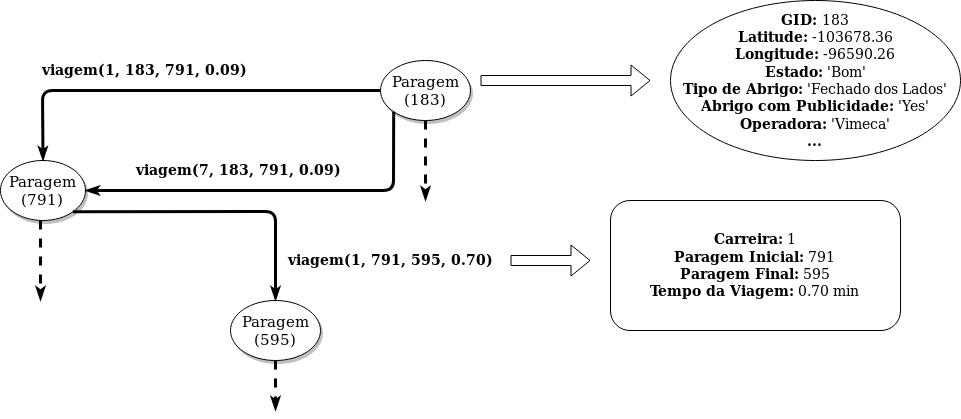
\includegraphics[scale = 0.45]{images/ExGrafo_SRCR.png}
    \caption{Exemplo básico do grafo do Sistema}
    \label{fig:ExGrafo_SRCR}
\end{figure}


\section{Algoritmos de Pesquisa}
\label{Algoritmos de Pesquisa}

\par Depois de termos uma noção do grafo final que iremos ter, será importante termos conhecimento de como os algoritmos de pesquisa aplicados na secção \ref{Aplicação dos Algoritmos de Procura}.
\par Neste trabalho foi tida em consideração 4 diferentes algoritmos de procura, sendo que 2 deles são por uma pesquisa \textbf{não informada (cega)} e o resto por pesquisas \textbf{informadas (através de uma heurística)}.
\par As pesquisas \textbf{não informadas} usam apenas as informações disponíveis na definição do problema. Pelo contrário, nas \textbf{informadas} dá-se ao algoritmo “dicas” sobre a adequação de diferentes estados.

\vspace{1cm}

\subsection{Procura primeiro em Largura (BFS)}
\label{Procura primeiro em Largura (BFS)}

O \textbf{BFS} garante que nenhum nodo é visitado mais que uma vez e, para isso acontecer, utiliza uma lista para garantir a ordem de chegada dos nodos. Assim, todos os nodos de menor profundidade são expandidos primeiro.
\par Este algoritmo de procura \textbf{não informada} costuma ter má performance para grafos muito grandes, como é o grafo deste problema. Para além disso, devido ao armazenamento dos nodos visitados, costuma ocupar muito espaço em memória. 
\par Por outro lado, este algoritmo chega sempre à solução ótima se o grafo tiver ramificação finita. 

\begin{figure}[H]
    \centering
    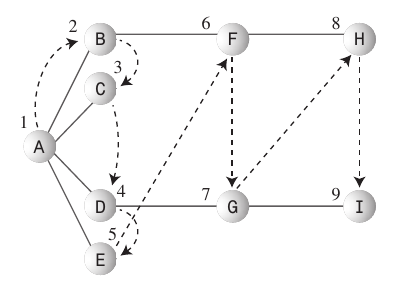
\includegraphics[scale = 0.8]{images/BFS.png}
    \caption{Procura primeiro em Largura}
    \label{fig:BFS}
\end{figure}

\vspace{5cm}

\subsection{Procura primeiro em Profundidade (DFS)}
\label{Procura primeiro em Profundidade (DFS)}

O algoritmo \textbf{DFS} (procura \textbf{não informada}) expande pelo primeiro nodo em profundidade até que encontre o nodo objetivo. Caso não o encontre, retrocede (\textit{backtrack}) e recomeça no próximo nodo.
\par A complexidade deste algoritmo é muito menor que a do \textbf{BFS} e ocupa menos memória.

\begin{figure}[H]
    \centering
    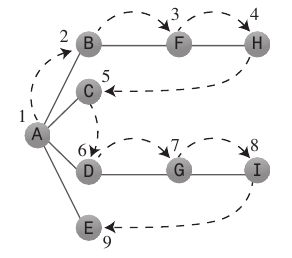
\includegraphics[scale = 0.8]{images/DFS.png}
    \caption{Procura primeiro em Profundidade}
    \label{fig:DFS}
\end{figure}

\vspace{20cm}

\subsection{Pesquisa Gulosa (Greedy Search)}
\label{Pesquisa Gulosa (Greedy Search)}

A pesquisa gulosa é um algoritmo de procura \textbf{informada} que expande os nodos consoante a heurística, fazendo a escolha ótima para a situação localizada na expansão daqueles nodos.
\par A pesquisa gulosa nem sempre produz a solução ótima, mas pode obter soluções relativamente perto do ótimo num período de tempo razoável.

\vspace{0.3cm}
\par Consideremos o exemplo em que se pretende chegar da cidade de Arad até Bucharest  através de um algoritmo de pesquisa gulosa (Russell and Norvig, 2009).

\begin{figure}[H]
    \centering
    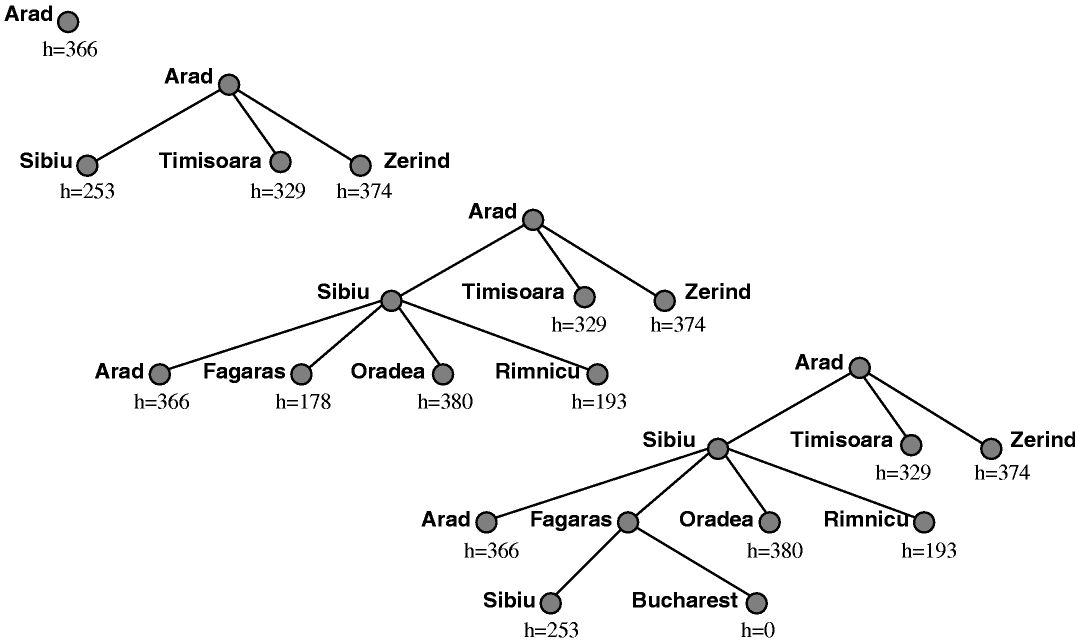
\includegraphics[scale = 0.35]{images/Greedy.png}
    \caption{Evolução da Pesquisa Gulosa}
    \label{fig:Greedy}
\end{figure}

Como podemos observar, o algoritmo tenta ir sempre pelo nodo com melhor heurística até chegar, se possível, ao nodo destino.

\vspace{10cm}

\subsection{Pesquisa A* (AEstrela)}
\label{Pesquisa A* (AEstrela)}

O algoritmo de pesquisa A* é semelhante ao da pesquisa gulosa. Este minimiza a soma do caminho já efetuado com o mínimo previsto que falta até a solução.
\par O A* é ótimo e completo, obtendo sempre a solução ótima

\vspace{0.3cm}
\par Consideremos o mesmo exemplo dado na pesquisa Gulosa, mas usando agora o algoritmo A*.

\begin{figure}[H]
    \centering
    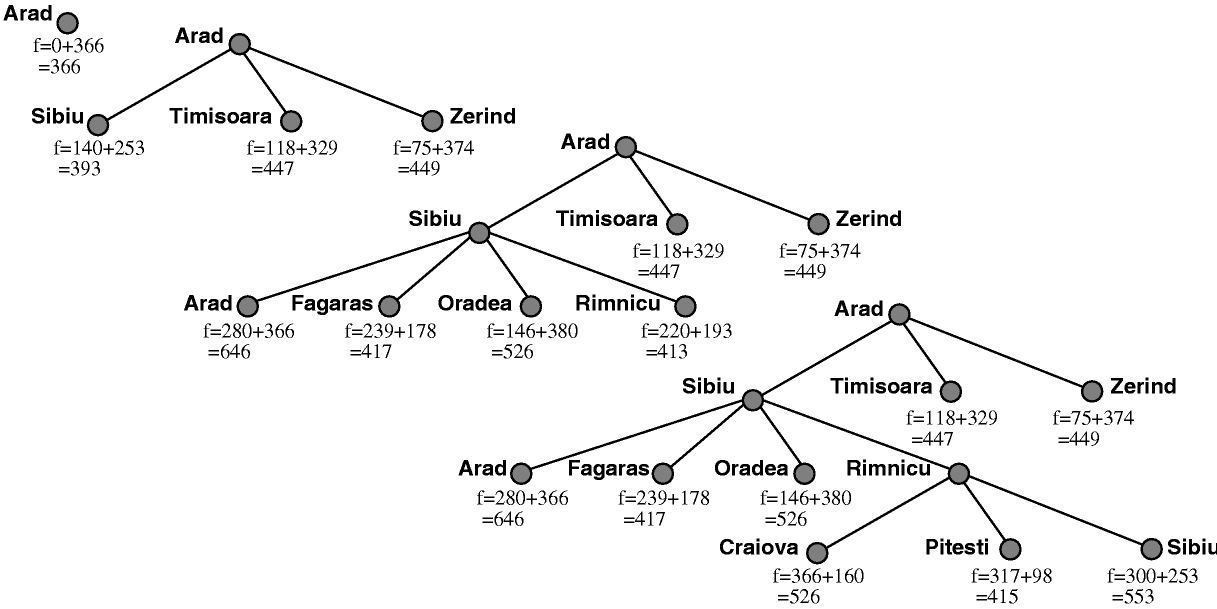
\includegraphics[scale = 0.35]{images/AEstrela.png}
    \caption{Evolução da Pesquisa A*}
    \label{fig:AEstrela}
\end{figure}



\chapter{Descrição do Trabalho e Análise de Resultados}
\label{Descrição do Trabalho e Análise de Resultados}

Primeiramente, procedeu-se a uma análise dos dados recolhidos e disponibilizados pelo concelho de Oeiras relativamente à área dos transportes públicos da região. Para isso, os documentos e dados fornecidos pela equipa docente demonstraram-se influentes no desenvolvimento do trabalho.
\par Após a análise dos dados, foi necessário uma limpeza destes devido à falta de valores e desformatação de alguns campos. Assim, é necessário realçar que os campos em falta foram preenchidos com \textbf{"N/A"}, de forma a representar a falta de informação. Esta falta de informação teve de ser verificada e corrigida numa fase posterior, ou seja, na fase de \textit{parse} dos dados e/ou nos algoritmos aplicados do próprio sistema.

\vspace{0.3cm}

\par Após a análise e limpeza dos dados, foi desenvolvido um programa em \textbf{Java} com o objetivo de aplicar um \textit{parse} aos dados dos ficheiros para depois termos em \textbf{PROLOG} predicados prontos a ser carregados para a base de conhecimento.

\vspace{20cm}

\section{Parse dos Dados em Java}

Tendo os dados relativos às paragens e lista de adjacências "limpos", procedeu-se ao desenvolvimento de um programa em \textbf{Java} para ler os vários ficheiros \textit{csv}\footnote{As várias folhas do ficheiro "lista\_adjacencias\_paragens"\hspace{0.0001cm} foram separadas em ficheiros diferentes com a extensão \textit{csv}.} e, após a correta separação da informação, escrever os predicados do \textbf{PROLOG} em ficheiros\footnote{Um ficheiro para as paragens e outro para as viagens, paragens.pl e viagens.pl respetivamente}. 

\par O programa desenvolvido em \textbf{Java} lê os dados dos vários ficheiros \textit{csv} provenientes do "lista\_adjacencias\_paragens"\footnote{\textbf{NOTA:} Apenas foi usado o ficheiro "lista\_adjacencias\_paragens" como forma de obter os dados para a resolução do trabalho}, organiza e escreve em dois ficheiros, mais tarde lidos pelo programa em \textbf{PROLOG}.


\vspace{0.5cm}

\par Assim, para cada ficheiro lido (num total de 39 que corresponde ao número de carreiras), o programa indica qual a paragem respetiva. 

\vspace{1cm}

\begin{verbatim}
// Para não haver paragens repetidas
if (!paragensId.contains(Integer.parseInt(data[0])))
{
    paragensId.add(Integer.parseInt(data[0]));

    paragem = "paragem(" + data[0] + ", " + data[1] + ", " + data[2]
    + ", '" + data[3] + "', '" + data[4] + "', '" + data[5] + "', '"
    + data[6] + "', " + data[8] + ", '" + data[9].replace("'", "")
    + "', '" + data[10].replace("\"", "") + "').";

    paragens.write(paragem + "\n");
}
\end{verbatim}

\vspace{0.5cm}

Desta forma, é possível fazer o \textit{parse} dos dados dos ficheiros e escrever o predicado da \textbf{paragem} como se pode observar de seguida:

\begin{verbatim}
:- dynamic paragem/10. 
paragem(183, -103678.36, -96590.26, 'Bom', 'Fechado dos Lados','Yes',
    'Vimeca', 286, 'Rua Aquilino Ribeiro', 'Carnaxide e Queijas').
paragem(791, -103705.46, -96673.6, 'Bom', 'Aberto dos Lados', 'Yes',
    'Vimeca', 286, 'Rua Aquilino Ribeiro', 'Carnaxide e Queijas').
paragem(595, -103725.69, -95975.2, 'Bom', 'Fechado dos Lados', 'Yes',
    'Vimeca', 354, 'Rua Manuel Teixeira Gomes', 'Carnaxide e Queijas').
paragem(182, -103746.76, -96396.66, 'Bom', 'Fechado dos Lados', 'Yes',
    'SCoTTURB', 286, 'Rua Aquilino Ribeiro', 'Carnaxide e Queijas').
...
\end{verbatim}

\vspace{5cm}

\par Do mesmo modo, as viagens também são obtidas durante a execução deste programa. Visto que o ficheiro lido possui a sequência de paragens que a carreira visita, sabemos que uma \textbf{viagem} pode ser obtida a partir desta sequência de paragens, como se observa de seguida:

\begin{verbatim}
String tempoViagem = pInicio.calculaTempo(pFim);

// viagem(carreira, paragemInicio, paragemFim, tempo de viagem).
viagem = "viagem(" + data[7] + ", " + pInicio.gid + ", " + pFim.gid
         + ", " + tempoViagem + ").";

if (iteracao > 1)
{
    viagens.write(viagem + "\n");
}
\end{verbatim}

\vspace{0.5cm}

\par É importante realçar que o parser para além escrever no predicado \textbf{viagem} a carreira e as duas paragens envolvidas, calcula desde já o tempo que está associado a esta viagem.

\par Este tempo, que também é calculado no \textbf{PROLOG} quando necessário \footnote{No \textbf{PROLOG} é necessário calculá-lo de forma a saber a heurística para os algoritmos informados.}, é obtido através da distância euclidiana das coordenadas das duas paragens:

\begin{verbatim}
double deltaLat = Math.pow((latF - latI), 2);  // em metros
double deltaLong = Math.pow((longF - longI), 2);  // em metros

// Resultado em minutos
return String.format(Locale.US, "%.2f",
    (Math.sqrt(deltaLat + deltaLong))/1000);
\end{verbatim}

Após o cálculo da distância euclidiana, é efetuada uma conversão desta distância em metros para minutos.\footnote{1 Km corresponde a 1 minuto.}

\vspace{0.5cm}
Assim sendo, otemos o predicado \textbf{viagem} da seguinte forma:
\begin{verbatim}
:- dynamic viagem/4. 
viagem(01, 183, 791, 0.09).
viagem(01, 791, 595, 0.70).
viagem(01, 595, 182, 0.42).
viagem(01, 182, 499, 2.00).
...
\end{verbatim}


\vspace{5cm}


\section{Aplicação dos Algoritmos de Procura}
\label{Aplicação dos Algoritmos de Procura}

Depois de obtidos os predicados fundamentais para a realização deste trabalho, a \textbf{paragem} e \textbf{viagem}, podemos começar a desenvolver os algoritmos de procura enunciados na secção \ref{Algoritmos de Pesquisa}. Estes algoritmos encontram-se definidos no ficheiro "algoritmosProcura.pl"\footnote{NOTA: A maioria dos algoritmos de pesquisa desenvolvidos seguiram metodologias das aulas práticas}.

\vspace{0.5cm}


\subsection{Pesquisa primeiro em Profundidade}

Para este algoritmo foram desenvolvidas duas versões do mesmo. Embora as duas tenham os mesmos resultados, uma permite calcular todas as possíveis soluções do algoritmo, sendo por isso mesmo, mais vezes usado, pois torna-se útil nas \textit{queries} desenvolvidas.



\begin{verbatim}
pesquisaProfundidade_varios(Origem,Destino,[(Origem,'Inicio')|Caminho],
TempoViagem) :-
    findall(
    paragem(Gid, Lat, Long, Estado, TipoAbrigo, Publicidade, Operadora,
        Codigo, NomeRua, Freguesia),
    paragem(Gid, Lat, Long, Estado, TipoAbrigo, Publicidade, Operadora, 
        Codigo, NomeRua, Freguesia),
    ListaParagens
    ),
    profundidade_func_varios(Origem, Destino, Caminho, TempoViagem,
        ListaParagens).
\end{verbatim}

\vspace{0.5cm}

\par Neste algoritmo, como é possível observar, é feito uma procura de todas as paragens das quais é possível percorrer ao procurar o caminho. Visto que esta chamada não é efetuada por nenhuma \textit{query} para uma procura mais restrita, qualquer paragem é aceite.
\par Podemos ver uma pesquisa mais restrita na seguinte função, chamada pela \textit{query} extra 10\footnote{Através do parâmetro 'Flag10'.}, que restringe a pesquisa a paragens que possuam bom estado de conservação.

\vspace{5cm}

\begin{verbatim}
pesquisaProfundidade_varios(Origem,Destino,[(Origem,'Inicio')|Caminho],
TempoViagem, 'Flag10') :-
    findall(
        paragem(G, L, Lo, 'Bom', T, Pub, Op, C, N, F),
        paragem(G, L, Lo, 'Bom', T, Pub, Op, C, N, F),
        ListaParagens
    ),
    profundidade_func_varios(Origem, Destino, Caminho, TempoViagem,
    	    ListaParagens).
\end{verbatim}

\vspace{0.5cm}

Para além de indicar o caminho, este algoritmo também calcula o tempo necessário para fazer a viagem. Este tempo é calculado através do parâmetro "Tempo de Viagem"\hspace{0.001cm} do predicado \textbf{viagem}. 
\par De realçar que para além do tempo de viagem entre cada paragem, foi adicionado um valor médio de 2 minutos que corresponde ao tempo de permanência em cada paragem. 
\vspace{0.3cm}
\par Outro aspeto a ter em conta é o facto que poderá haver ocorrência de valores indefinidos ("N/A") no tempo entre viagens, pelo que, terá de ser ajustado. A forma considerada para o sistema se comportar nestas situações foi a consideração que o valor do tempo seria 0, ou seja, não afetaria o valor já calculado.

\begin{verbatim}
profundidade_func_varios(Paragem,Destino,[(ProxParagem, Carreira)|Caminho], 
    TempoViagem, ListaParagens) :- 
    adjacente(Paragem, ProxParagem, Carreira, T1, ListaParagens),
    ((T1 == 'N/A') -> TLimpo is 0.0 ; TLimpo is T1),
    profundidade_func_varios(ProxParagem, Destino, Caminho, T, 
        ListaParagens),
    TempoViagem is T + TLimpo + 2.                          
\end{verbatim}

\vspace{1cm}

Resultado de uma procura em profundidade entre a paragem 183 e a 608. O caminho da solução tem o par da paragem e a respetiva carreira da viagem.

\begin{verbatim}
| ?- pesquisaProfundidade_varios(183, 608, Caminho, Tempo).
Caminho = [(183,'Inicio'),(791,1),(595,1),(182,1),(499,1),
    (593,1),(181,1),(180,1),(594,1),(...,...)|...],
Tempo = 68.84 ? ;
Caminho = [(183,'Inicio'),(791,1),(595,1),(182,1),(499,1),
    (593,1),(181,1),(180,1),(594,1),(...,...)|...],
Tempo = 68.84 ? 
yes
\end{verbatim}

\vspace{10cm}

\subsection{Pesquisa primeiro em Largura}

Tal como no algoritmo de pesquisa em profundidade, o de largura também tem duas versões. Contudo, estas duas versões diferem simplesmente no \textit{output}, sendo que um devolve um caminho com mais informações relativas às paragens que o outro.


\begin{verbatim}
pesquisaLarguraSimplificado(Origem, Destino, Caminho) :-
    findall(
    paragem(Gid, Lat, Long, Estado, TipoAbrigo, Publicidade,
        Operadora, Codigo, NomeRua, Freguesia),
    paragem(Gid, Lat, Long, Estado, TipoAbrigo, Publicidade,
        Operadora, Codigo, NomeRua, Freguesia),
    ListaParagens
    ),
    pesquisaLarguraSimplificado_fun([[(Origem, 'Inicio')]],
        Destino, C, ListaParagens),
    inverso(C, Caminho).
\end{verbatim}  

\par Este algoritmo apenas difere do anterior pela forma como expande o grafo.

\begin{verbatim}
| ?- pesquisaLarguraSimplificado(183, 595, Caminho).
Caminho = [(183,'Inicio'),(791,1),(595,1)] ? ;
Caminho = [(183,'Inicio'),(791,1),(595,7)] ? ;
Caminho = [(183,'Inicio'),(791,1),(595,10)] ? 
yes
\end{verbatim}

\vspace{1cm}

\subsection{Pesquisa A*}

Para o desenvolvimento do algoritmo de A*, a existência do tempo como parâmetro no predicado \textbf{viagem} permitiu poupar alguns dos cálculos que envolviam as heurísticas.

\par Mesmo assim foi necessário desenvolver uma função que permitisse determinar a heurística tendo em conta duas paragens.

\begin{verbatim}
tempoEstimado((LatX, LongX), (LatY, LongY), Estima) :- 
    ((LatX == 'N/A') -> LatLimpoX is 999.9; LatLimpoX is LatX),
    ((LongX == 'N/A') -> LongLimpoX is 999.9; LongLimpoX is LongX),
    ((LatY == 'N/A') -> LatLimpoY is 999.9; LatLimpoY is LatY),
    ((LongY == 'N/A') -> LongLimpoY is 999.9; LongLimpoY is LongY),
    DeltaLat is LatLimpoX - LatLimpoY,
    DeltaLong is LongLimpoX - LongLimpoY,
    Estima is (sqrt(DeltaLat^2 + DeltaLong^2))/1000.
\end{verbatim}

\par Desta forma, é necessário realçar que caso fossem encontrados valores indefinidos ("N/A"), ter-se-ia de substituir o seu valor. Neste caso o valor 999.9 pareceu o mais adequado para o cálculo da distância.

\par Desta forma, temos tudo para podermos implementar o algoritmo de procura informada.

\begin{verbatim}
pesquisaAEstrela(Origem, Destino, Caminho, Tempo) :-            
    findall(
    paragem(Gid, Lat, Long, Estado, TipoAbrigo, 
        Publicidade, Operadora, Codigo, NomeRua, Freguesia),
    paragem(Gid, Lat, Long, Estado, TipoAbrigo, 
        Publicidade, Operadora, Codigo, NomeRua, Freguesia),
    ListaParagens
    ),
    resolve_aestrela((Origem, 'Inicio'), Destino,
        Caminho/Tempo, ListaParagens).
        
...

obtem_melhor([Caminho1/Tempo1/Est1, _/Tempo2/Est2|Caminhos],
MelhorCaminho) :-
	Tempo1 + Est1 =< Tempo2 + Est2, !,
	obtem_melhor([Caminho1/Tempo1/Est1|Caminhos], MelhorCaminho).
\end{verbatim}

É também importante realçar esta última função que calcula o custo (tempo) acumulado da melhor solução que passa por esta paragem (nodo).


\vspace{0.7cm}

\subsection{Pesquisa Gulosa}

O algoritmo da pesquisa gulosa é muito semelhante ao pesquisa A*, pelo que consequentemente as funções que o aplicam também são em tudo semelhantes.

\begin{verbatim}
pesquisaGulosa(Origem, Destino, Caminho, Tempo) :-            
    findall(
    paragem(Gid, Lat, Long, Estado, TipoAbrigo,
        Publicidade, Operadora, Codigo, NomeRua, Freguesia),
    paragem(Gid, Lat, Long, Estado, TipoAbrigo, Publicidade,
        Operadora, Codigo, NomeRua, Freguesia),
    ListaParagens
    ),
    resolve_gulosa((Origem, 'Inicio'), Destino,
        Caminho/Tempo, ListaParagens).   
\end{verbatim}

\par Contudo, a pesquisa gulosa difere da pesquisa A* na forma de comparação das heurísticas, visto que não acumula o tempo.
\par Logo, temos a seguinte função:

\begin{verbatim}
obtem_melhor_gulosa([Caminho1/Tempo1/Est1, _/_/Est2|Caminhos],
MelhorCaminho) :-
	Est1 =< Est2, !,
	obtem_melhor_gulosa([Caminho1/Tempo1/Est1|Caminhos],
	    MelhorCaminho).
\end{verbatim}

\par Como podemos observar, a função apenas difere na comparação das estimas (heurística).

\section{Funcionalidades do Sistema}

De forma a demonstrar as funcionalidades do sistema desenvolvido, era pretendido implementar um conjunto de requisitos propostos pela equipa docente que incidiam diferentes formas de aplicação dos algoritmos desenvolvidos.
\par Assim, irão ser enumeradas as várias funcionalidades realizadas, bem como os seus resultados.


\subsection{Funcionalidade 1}
\begin{itemize}
    \item \textbf{Calcular um trajeto entre dois pontos}
\end{itemize} 
\par Esta funcionalidade apenas necessita da determinação do trajeto a percorrer, logo apenas precisámos de invocar um algoritmos de procura.
\par Deste modo, foram disponibilizadas várias alternativas relativamente ao algoritmo usado, sendo possível executá-la consoante algoritmos diferentes e comparar os resultados obtidos.


\begin{verbatim}
trajetoEntre2Pontos(Origem, Destino, 'Profundidade') :-   
    pesquisaProfundidade_varios(Origem, Destino, Caminho,
        TempoViagem), 
    printCaminhoTempo(Caminho, TempoViagem).

trajetoEntre2Pontos(Origem, Destino, 'AEstrela') :-
    pesquisaAEstrela(Origem, Destino, Caminho, Tempo),
    printCaminhoTempo(Caminho, Tempo).
\end{verbatim}

Neste excerto de código, podemos observar que é possível executar a funcionalidade com diferentes algoritmos\footnote{É possível executar os 4 algoritmos de procura falados anteriormente na secção \ref{Algoritmos de Pesquisa}. Também é permitido usar diferentes versões nos algoritmos de procura não informada.}, que possibilita diferentes resultados entre eles.

\vspace{0.5cm}

\par Segue-se o resultado do uso desta funcionalidade:

\begin{verbatim}
| ?- trajetoEntre2Pontos(183, 180, 'Profundidade').   
Trajeto efetuado: 
        Paragem: 183
         -> Carreira Inicio
        Paragem: 791
         -> Carreira 1
        Paragem: 595
         -> Carreira 1
        Paragem: 182
         -> Carreira 1
        Paragem: 499
         -> Carreira 1
        Paragem: 593
         -> Carreira 1
        Paragem: 181
         -> Carreira 1
        Paragem: 180
         -> Carreira 1
        Tempo de Viagem -> 19.319999999999997 minutos
yes
\end{verbatim}

\par Assim, o trajeto entre a paragem 183 e a 180 tem uma duração de 19 minutos\footnote{De notar que já está incluído o tempo de espera de 5 minutos entre viagens.} percorrendo um total de 8 paragens. Apenas foi usada a carreira 1 para este trajeto.

\vspace{1cm}

\subsection{Funcionalidade 2}
\begin{itemize}
    \item \textbf{Selecionar apenas algumas das operadoras de transporte para um determinado percurso}
\end{itemize}
\par Nesta funcionalidade, é pedido que limitemos o número de paragens às quais o trajeto pode passar. Por isso mesmo, invocamos o algoritmo de pesquisa em profundidade, mas limitado às operadoras introduzidas.
\par A pesquisa de profundidade irá então verificar quais as paragens às quais pode passar consoante as operadoras e, depois, irá calcular o trajeto.


\begin{verbatim}
trajetoCertasOperadoras(Origem, Destino, Caminho, TempoViagem,
Operadoras) :-    
    pesquisaProfundidade_varios(Origem, Destino, Caminho, TempoViagem,
        Operadoras),
    printCaminhoTempo(Caminho, TempoViagem).
    

| ?- trajetoCertasOperadoras(183, 595, Caminho, TempoViagem, ['Carris']).
no
| ?- trajetoCertasOperadoras(183, 595, Caminho, TempoViagem, ['Vimeca']).
Trajeto efetuado: 
        Paragem: 183
         -> Carreira Inicio
        Paragem: 791
         -> Carreira 1
        Paragem: 595
         -> Carreira 1
        Tempo de Viagem -> 4.79 minutos
Caminho = [(183,'Inicio'),(791,1),(595,1)],
TempoViagem = 4.79 ? 
yes
| ?-
\end{verbatim}

\par Como podemos observar, se tentarmos calcular o trajeto entre duas paragens que não possuam a operadora selecionada ("Carris"), não obtemos nenhum resultado, pois tal não é possível.
\par Contudo, se introduzirmos operadoras presentes nas paragens, conseguimos determinar um trajeto a percorrer.

\vspace{1cm}

\subsection{Funcionalidade 3}
\begin{itemize}
    \item \textbf{Excluir um ou mais operadores de transporte para o percurso}
\end{itemize}

\par Esta funcionalidade funciona de maneira muito semelhante à anterior, pelo que a lógica usada também o é.
\par Visto que estamos a excluir operadoras, necessitamos de determinar quais as operadoras que podemos usar para percorrer o trajeto. 
\par Desta forma, é usado um \textit{findall} seguido de um \textit{sort} para identificarmos as operadoras possíveis, ou seja, todas excepto as introduzidas como parâmetro. Já o \textit{sort} apresenta-as numa lista sem repetidos. 
\par De seguida, invocamos a função de pesquisa em profundidade para o cálculo do trajeto.

\begin{verbatim}
trajetoSemCertasOperadoras(Origem, Destino, Caminho, TempoViagem,
Operadoras) :-
    findall(
        Op,
        (paragem(_, _, _, _, _, _, Op, _, _, _), 
            \+ member(Op, Operadoras)),
        ListaOpt
    ),
    sort(ListaOpt, OperadorasPossiveis),                               
    pesquisaProfundidade_varios(Origem, Destino, Caminho,
        TempoViagem, OperadorasPossiveis),
    printCaminhoTempo(Caminho, TempoViagem).
\end{verbatim}

\vspace{0.5cm}

\par Esta funcionalidade tem os seguintes resultados:

\begin{verbatim}
| ?- trajetoSemCertasOperadoras(183, 595, Caminho, TempoViagem,
    ['Carris']).
Trajeto efetuado: 
        Paragem: 183
         -> Carreira Inicio
        Paragem: 791
         -> Carreira 1
        Paragem: 595
         -> Carreira 1
        Tempo de Viagem -> 4.79 minutos
Caminho = [(183,'Inicio'),(791,1),(595,1)],
TempoViagem = 4.79 ? 
yes
| ?- trajetoSemCertasOperadoras(183, 595, Caminho, TempoViagem,
    ['Vimeca']).
no
\end{verbatim}

\par Como era esperado, o resultado desta funcionalidade é inverso ao da anterior.

\vspace{1cm}

\subsection{Funcionalidade 4}
\begin{itemize}
    \item \textbf{Identificar quais as paragens com o maior número de carreiras num determinado percurso}
\end{itemize}

\par O ideologia desta funcionalidade consiste em calcular o trajeto entre duas paragens, como é feito anteriormente, mas, após esse cálculo, é determinado para cada paragem o número de carreiras que esta possui através de um \textit{findall}\footnote{Usado na função "calculaCarreiras".}.
\par De seguida, é apresentada a paragem que possui o maior número de carreiras.

\begin{verbatim}
paragemMaisCarreiras(Origem, Destino) :-
    pesquisaProfundidade_varios(Origem, Destino, Caminho, 
        TempoViagem),
    printCaminhoTempo(Caminho, TempoViagem),
    nl, write('----------------'), nl, nl,
    write('Paragem com mais carreiras...'), nl, nl,
    calculaCarreiras(Caminho, (Paragem, NumCarreiras)),
    write('Paragem -> '), format('~w', Paragem), nl,
    write('Numero de Carreiras -> '), format('~w', NumCarreiras),
    nl,
    write('\tTempo -> '), format('~w', TempoViagem).
\end{verbatim}  

\vspace{0.5cm}

\par Resultado desta funcionalidade:

\begin{verbatim}
| ?- paragemMaisCarreiras(183, 182).
Trajeto efetuado: 
        Paragem: 183
         -> Carreira Inicio
        Paragem: 791
         -> Carreira 1
        Paragem: 595
         -> Carreira 1
        Paragem: 182
         -> Carreira 1
        Tempo de Viagem -> 7.21 minutos

----------------

Paragem com mais carreiras...

Paragem -> 595
Numero de Carreiras -> 7
        Tempo -> 7.21
yes
\end{verbatim}

\par Assim, no trajeto entre a paragem 183 e 182, a paragem que possui mais carreiras é a 595 com 7 Carreiras.

\vspace{1cm}

\subsection{Funcionalidade 5}
\begin{itemize}
    \item \textbf{Escolher o menor percurso (usando critério menor número de paragens)}
\end{itemize}

\par A ideologia da resolução desta funcionalidade consiste na determinação de todos os caminhos possíveis entre as duas paragens através do \textit{findall} da função de pesquisa em profundidade.
\par Esta funcionalidade só funciona com a pesquisa em profundidade, pois os outros algoritmos, da maneira que estão definidos, não permitem o cálculo de todos caminhos possíveis.
\par Após o cálculo de todos trajetos, é preciso determinar qual apresenta menor número de paragens e apresentá-lo.

\begin{verbatim}
menorPercurso(ParagemInicio, ParagemFim, Caminho, NParagens) :-
    findall(
        (Caminho, L),
        (pesquisaProfundidade_varios(ParagemInicio, ParagemFim,
            Caminho, _), length(Caminho, L)),
        ListaCaminho
    ),
    menosParagens(ListaCaminho, ([], 9999.9), (Caminho, NParagens)). 
\end{verbatim}      

\vspace{0.5cm}

Segue-se um resultado desta funcionalidade:

\begin{verbatim}
| ?- menorPercurso(183, 595, Caminho, NumeroParagens).
Paragem -> 183,Inicio
Paragem -> 791,15
Paragem -> 595,15
Caminho = [(183,'Inicio'),(791,15),(595,15)],
NumeroParagens = 3 ? 
yes
\end{verbatim} 

\par Deste modo, o melhor caminho consoante o número de paragens entre 183 e 595 é o seguinte, com 3 paragens.

\vspace{1cm}

\subsection{Funcionalidade 6}
\begin{itemize}
    \item \textbf{Escolher o percurso mais rápido (usando critério da distância)}
\end{itemize}

\par Visto que era pretendido usar o critério da distância, foi usado o algoritmo da pesquisa A*. Este algoritmo apresenta a heurística em tempo (minutos), mas visto que foi usada uma correspondência de 1 Km para 1 minuto, o trajeto com menor tempo é necessariamente o trajeto com menor distância.


\begin{verbatim}
trajetoMaisRapido(Origem, Destino) :-
    pesquisaAEstrela(Origem, Destino, Caminho, Tempo),
    printCaminhoTempo(Caminho, Tempo).
\end{verbatim}

O resultado desta funcionalidade pode ser o seguinte:

\begin{verbatim}
| ?- trajetoMaisRapido(183, 182).
Trajeto efetuado: 
        Paragem: 183
         -> Carreira Inicio
        Paragem: 791
         -> Carreira 1
        Paragem: 595
         -> Carreira 1
        Paragem: 182
         -> Carreira 1
        Tempo de Viagem -> 7.21 minutos
yes
\end{verbatim}


\vspace{10cm}

\subsection{Funcionalidade 7}
\begin{itemize}
    \item \textbf{Escolher o percurso que passe apenas por abrigos com publicidade}
\end{itemize}

\par Esta funcionalidade requeria um filtro das paragens que seria possível percorrer. Por isso mesmo, foi chamada uma função de pesquisa em profundidade que restringe as paragens possíveis às que têm publicidade. 
\par Esta função é identificada pelo parâmetro "Flag7"\hspace{0.001cm} que identifica a função para a funcionalidade 7.

\begin{verbatim}
trajetoAbrigosPub(Origem, Destino) :-
    pesquisaProfundidade_varios(Origem, Destino, Caminho,
        Tempo, 'Flag7'),
    printCaminhoTempo(Caminho, Tempo).
\end{verbatim}

\vspace{0.5cm}

Seguem-se possíveis os resultados:

\begin{verbatim}
| ?- trajetoAbrigosPub(180, 185).
no
| ?- trajetoAbrigosPub(183, 182).
Trajeto efetuado: 
        Paragem: 183
         -> Carreira Inicio
        Paragem: 791
         -> Carreira 1
        Paragem: 595
         -> Carreira 1
        Paragem: 182
         -> Carreira 1
        Tempo de Viagem -> 7.21 minutos
yes
\end{verbatim}

\par Visto que o trajeto entre as paragens 180 e 185 precisa de passar pela paragem 594, que não possui publicidade, este não é possível.
\par Por outro lado, o trajeto entre 183 e 182 é possível, pois todas as paragens cumprem o requisito.

\vspace{10cm}

\subsection{Funcionalidade 8}
\begin{itemize}
    \item \textbf{Escolher o percurso que passe apenas por paragens abrigadas}
\end{itemize}
\par Para a realização desta funcionalidade foi introduzida a mesma lógica usada anteriormente, ou seja, foram feitas filtragens das paragens que seriam possíveis percorrer e, a partir destas, foi determinado o trajeto a percorrer.

\begin{verbatim}
trajetoParagemAbrigada(Origem, Destino) :-
    findall(
        Abrigo,
        (paragem(_, _, _, _, Abrigo, _, _, _, _, _),
            Abrigo \== 'Sem Abrigo', Abrigo \== 'N/A'),
        ListaComAbrigo
    ),
    sort(ListaComAbrigo, ParagensComAbrigo),                       
    pesquisaProfundidade_varios(Origem, Destino, Caminho,
        Tempo, ParagensComAbrigo, 'Flag8'),
    printCaminhoTempo(Caminho, Tempo).
\end{verbatim}

\par É importante realçar que, caso existam paragens sem informação do seu abrigo, estes são \textbf{rejeitados} pela função, ou seja, não podem ser percorridos.
\par Por isso mesmo, no \textit{findall} são vistos todos os abrigos que existem no sistema e que não sejam "Sem Abrigo"\hspace{0.001cm} ou "N/A"\hspace{0.001cm} (indefinidos).

\begin{verbatim}
| ?- trajetoParagemAbrigada(593, 180).
no
| ?- trajetoParagemAbrigada(89, 597).
Trajeto efetuado: 
        Paragem: 89
         -> Carreira Inicio
        Paragem: 107
         -> Carreira 1
        Paragem: 250
         -> Carreira 1
        Paragem: 261
         -> Carreira 1
        Paragem: 597
         -> Carreira 1
        Tempo de Viagem -> 9.920000000000002 minutos
yes
\end{verbatim}

\par Como podemos observar, caso o trajeto tenha de passar por paragens não abrigadas, este não é aceite\footnote{A paragem 593 não possui abrigo.}.


\vspace{5cm}

\subsection{Funcionalidade 9}
\begin{itemize}
    \item \textbf{Escolher um ou mais pontos intermédios por onde o percurso deverá passar}
\end{itemize}

\par Esta funcionalidade requer que sejam calculados todos os caminhos possíveis entre as duas paragens e, após esse cálculo, escolher um que tenha os pontos intermédios pretendidos.
\par Assim, esta funcionalidade precisa no mínimo de um ponto intermédio para determinar um caminho, ou seja, caso não receba nenhum, não irá apresentar o trajeto.

\begin{verbatim}
trajetoComPontosInterm(Origem, Destino, Interm) :-
    findall(
        Caminho,
        (pesquisaProfundidade_varios(Origem, Destino,
            Caminho, _)),
        ListaCaminho
    ),
    Interm \= [],
    tiraCarreirasList(ListaCaminho, [], NovaListaCaminho),
    intermedioLista(NovaListaCaminho, [], L),
    temInterm(L, Interm, CaminhoEscolhido),
    printParagem(CaminhoEscolhido).
\end{verbatim} 

\par Como é observável, após o \textit{findall} dos caminhos, é usada uma função para verificar e dar como output um caminho que tenha os pontos intermédios pretendidos.
Para isso é verificado se o caminho tem como sub-lista o conjunto dos pontos intermédios.

\begin{verbatim}
| ?- trajetoComPontosInterm(183, 595, [791]).
Paragem -> 183
Paragem -> 791
Paragem -> 595
yes
| ?- trajetoComPontosInterm(183, 595, [121]).
no
| ?- trajetoComPontosInterm(183, 595, []).
no
\end{verbatim}  

\par Neste exemplo, o trajeto entre 183 e 595 passando por 121 ou passando por nenhuma paragem intermédia é impossível, pelo que dá \textit{no}. 
\par Contudo, se passar pela paragem 791 já é possível.

\vspace{10cm}

\subsection{Funcionalidade 10 (Extra)}
\par Para além das funcionalidades pedidas pela equipa docente foram desenvolvidas duas extra de forma a demonstrar melhor as possibilidades do sistema.

\vspace{1cm}

\begin{itemize}
    \item \textbf{Escolher um percurso que passe apenas por paragens em Bom estado de conservação}
\end{itemize}

\par Esta funcionalidade possui um raciocínio muito semelhante aos anteriores na forma de obtenção do trajeto.
\par Deste modo, foi feito uma filtragem das paragens que apresentavam um bom nível de conservação e, de seguida, determinado um caminho possível entre as paragens.

\begin{verbatim}
trajetoParagemBomEst(Origem, Destino) :-
    pesquisaProfundidade_varios(Origem, Destino, Caminho,
        Tempo, 'Flag10'),
    printCaminhoTempo(Caminho, Tempo).
\end{verbatim}  

Um possível resultado seria o seguinte:

\begin{verbatim}
| ?- trajetoParagemBomEst(183, 595).
Trajeto efetuado: 
        Paragem: 183
         -> Carreira Inicio
        Paragem: 791
         -> Carreira 1
        Paragem: 595
         -> Carreira 1
        Tempo de Viagem -> 4.79 minutos
yes
\end{verbatim}  

Todas as paragens deste trajeto apresentam bom estado de conservação.

\vspace{10cm}

\subsection{Funcionalidade 11 (Extra)}
\begin{itemize}
    \item \textbf{Trajeto entre duas ruas}
\end{itemize}

\par Nesta funcionalidade, em vez de inserirmos o identificador de duas paragens, são introduzidos a rua em que a pessoa está e a rua para onde se pretende deslocar. 
\par De seguida, seria calculado o trajeto a seguir para a deslocação entre essas duas ruas.

\begin{verbatim}
trajetoEntreDuasRuas(RuaOrigem, RuaDestino) :-
    paragem(Origem, _, _, _, _, _, _, _, RuaOrigem, _),
    paragem(Destino, _, _, _, _, _, _, _, RuaDestino, _),
    pesquisaProfundidade_varios(Origem, Destino, Caminho, Tempo),
    printCaminhoTempo(Caminho, Tempo).
| ?- trajetoEntreDuasRuas('Rua Aquilino Ribeiro', 'Avenida dos Cavaleiros').
Trajeto efetuado: 
        Paragem: 183
         -> Carreira Inicio
        Paragem: 791
         -> Carreira 1
        Paragem: 595
         -> Carreira 1
        Paragem: 182
         -> Carreira 1
        Paragem: 499
         -> Carreira 1
        Tempo de Viagem -> 11.21 minutos
yes
\end{verbatim}  


\vspace{30cm}
\section{Análise e Comparação de Resultados}

\par Devido à existência de algoritmos de procura diferentes, num conceito de utilização real, a escolha do algoritmo mais adequado torna-se muito importante a nível de memória e, principalmente, performance.
\par Neste trabalho foram desenvolvidos 4 algoritmos de procura diferentes. Durante a realização das funcionalidades, alguns algoritmos mostraram-se mais eficientes que outros devido aos requisitos impostos e à procura que era pretendida.
\par A nível teórico e em certas situações, o algoritmo de pesquisa em profundidade (DFS) mostra-se mais eficiente a encontrar uma solução em comparação ao resto. Contudo, quando se pretende a solução ótima, os algoritmos de pesquisa informada mostram-se superiores, principalmente se a heurística usada for boa. 
\par Entre o A* e a gulosa, a gulosa tende a ter resultados mais rápidos, embora não garanta a solução ótima ao contrário da A*.

\vspace{0.5cm}
\par De forma a demonstrar isto a nível prático, foram feitos alguns testes de procuras e mediu-se o tempo de execução através do predicado \textit{statistics}.

\begin{verbatim}
| ?- trajetoEntre2Pontos(183, 595, 'Profundidade', TempoExecucao). 
...
TempoExecucao = 0 ? yes
| ?- trajetoEntre2Pontos(183, 595, 'LarguraSimplificado', TempoExecucao).
...
TempoExecucao = 270 ? 
yes
| ?- trajetoEntre2Pontos(183, 595, 'AEstrela', TempoExecucao).
...
TempoExecucao = 280 ? 
yes
| ?- trajetoEntre2Pontos(183, 595, 'Gulosa', TempoExecucao).
...
TempoExecucao = 80 ? 
yes
\end{verbatim}  

Como é possível observar, a pesquisa em profundidade tem uma melhor performance (aproximadamente 0 milissegundos), derivada da estrutura do grafo e do caminho pedido. A largura tem uma performance muito inferior e muito semelhante à procura A* (270 e 280 milissegundos, respetivamente). Por último, a pesquisa gulosa surge em melhor posição que a A*, tal como era esperado (80 milissegundos).
\vspace{0.5cm}
\par Desta forma, podemos verificar que os resultados na prática dos algoritmos se encontram da forma esperada pela teoria.
\vspace{0.5cm}
\par É importante salientar que as limitações impostas pelo \textbf{PROLOG} não permitiram testar os algoritmos com mais exaustão, pelo que não conseguimos comparar os algoritmos e as funcionalidades da maneira desejada.


\chapter{Conclusão e Sugestões}

Em suma, com este trabalho foi possível aplicar na prática todos os conhecimentos adquiridos nas aulas relativamente à resolução de problemas e no desenvolvimento de algoritmos de pesquisa através da linguagem lógica (\textbf{PROLOG}).
\par Além disso, pudemos transpor predicados sugeridos nas aulas práticas e teóricas que possibilitaram o desenvolvimento de algoritmos estudados.
\par Assim, acho que foram cumpridos todos os objetivos propostos pela equipa docente para a realização deste trabalho, que se revelou muito interessante, principalmente pelo facto que utilização de dados reais permitiu ter uma noção do tipo de trabalho que nos tem pela frente.
\par Contudo, considero que o relatório do trabalho ficou demasiado extenso devido à necessidade de descrição do trabalho feito, de forma a possibilitar uma melhor percepção da metodologia de trabalho aplicada.







\begin{thebibliography}{}
\bibitem{}
Russell and Norvig, (2009) Artificial Intelligence -A Modern Approach.
\bibitem{}
Bratko I. (1986). Prolog programming for artificial intelligence. Wokingham: Addison-Wesley.
\bibitem{}
Município de Oeiras - Dados Abertos Municipais.     
\url{https://dados.geomunicipio.org/fa_IR/dataset/paragens-de-autocarro}
\end{thebibliography}



\end{document}











